\documentclass[11pt]{article}

\usepackage{authblk}
\usepackage{fullpage}
\usepackage{color}
\usepackage{amsmath,amsfonts,amssymb}
\usepackage{threeparttable}% tables with footnotes
\usepackage{dcolumn}% decimal-aligned tabular math columns
\usepackage{hyperref}
\usepackage{subfigure}
\usepackage{graphicx}
%\hypersetup{colorlinks=false,
%                       linkbordercolor={1 1 1}}
\hypersetup{bookmarks=true,
colorlinks=true,
linkcolor=black,
citecolor=black,
filecolor=black,
pagecolor=blue,
urlcolor=black,
plainpages=false,
}

\graphicspath{{figs/}}                                                          

% New Commands
%========================================================================
\newcommand{\mbb}[1]{\mathbb{#1}}
\newcommand{\mbf}[1]{\mathbf{#1}}
\newcommand{\sbf}[1]{\boldsymbol{#1}}
\newcommand{\mcal}[1]{\mathcal{#1}}
\newcommand{\mfk}[1]{\mathfrak{#1}}
\newcommand{\pp}[2]{\frac{\partial #1}{\partial #2}}
\newcommand{\dd}[2]{\frac{d #1}{d #2}}
\newcommand{\rarrow}{\rightarrow}
\newcommand{\Rarrow}{\Rightarrow}
\newcommand{\LRarrow}{\Leftrightarrow}
\newcommand{\jump}[1]{\llbracket #1 \rrbracket}
\newcommand{\avg}[1]{\{ #1 \}}
\def\etal{{\it et al.~}}
\newcommand{\vvvert}{|\kern-1pt|\kern-1pt|}
\newcommand{\enorm}[1]{\vvvert #1 \vvvert}
\newcommand{\ud}{\,\mathrm{d}}
\newcommand{\sa}{\nu_{\mathrm{sa}}}
\newcommand{\sao}{m}
\newcommand{\tsa}{\mathrm{sa}}
\newcommand{\brho}{\bar{\rho}}
\newcommand{\bp}{\bar{p}}
\newcommand{\bq}{\bar{q}}
\newcommand{\tu}{\tilde{u}}
\newcommand{\tv}{\tilde{v}}
\newcommand{\tS}{\tilde{S}}
\newcommand{\tE}{\tilde{E}}
\newcommand{\bmu}{\bar{\mu}}
\newcommand{\hh}{\tilde{h}}

%========================================================================
                                                                         
% Title Stuff
%========================================================================
\title{Model Document: Predictive Validation Oscillator Example}

\author{Todd A. Oliver, Gabriel Terejanu, Robert D.~Moser, and Chris Simmons}
\affil{Center for Predictive Engineering and Computational Sciences,\\
Institute for Computational Engineering and Sciences,\\
The University of Texas at Austin, Austin TX, 78712,\\
{\tt oliver@ices.utexas.edu}}

% Document starts here
%========================================================================
\begin{document}
\maketitle

\begin{abstract}
This document describes a simple application of the predictive
validation methodology.
\end{abstract}

\section{Brief Problem Description}
We will use the predictive validation methodology to examine a toy
problem involving a mass-spring-damper system.  In the toy problem, we
will be given a handful of observations of the position of the mass at
particular times for two different masses.  We wish to use the
observations to validate a model to predict the maximum velocity of a
larger mass.

\section{Physical Model and Required Prediction}
\label{sec:phys_model}
A notional depiction of the physical system is shown in Figure~\ref{fig:smd_sys}.
%
\begin{figure}[ht]
\begin{center}
\includegraphics[width=0.3\linewidth]{smd_sys.pdf}
\end{center}
\caption{The spring-mass-damper system of interest.}
\label{fig:smd_sys}
\end{figure}
%
Newton's second law requires that
%
\begin{equation}
m \ddot{x} = f_d + f_s,
\label{eqn:fma}
\end{equation}
% 
where $m$ is the mass, $x$ is the position of the mass, and $f_d$ and
$f_s$ are the forces acting on the mass due to the damper and the
spring, respectively.  We assume that any other forces acting on the
mass (e.g., drag, gravity) are known to have negligible effect.  Thus,
\eqref{eqn:fma} represents highly reliable theory in the context of
the current problem.  However, $f_d$ and $f_s$ must be specified.
Thus, we require embedded, potentially inadequate, models for these
forces.

For simplicity, we choose to use typical linear models for both the spring
and the damper.  Thus, the embedded models are
%
\begin{align*}
f_s &= -k x, \\
f_d &= -c_o \dot{x},
\end{align*}
%
where the parameters $k$ and $c_o$ are unknown.

We wish to use this model to predict the maximum velocity of the mass
for $m=5$ with an initial condition of $x(0) = 4$, $\dot{x}(0) = 0$.


\section{``True'' Physical System}
\label{sec:true_phys_sys}
For the purposes of this exercise, only two aspects of the actual
system are relevant: 1.) any observations of it that are available for
calibration and validation purposes and 2.) any knowledge that we
have regarding the relationship between our model and the truth.
These items are discussed here.  The actual system used to generate
the truth data is detailed in Appendix~\ref{app:truth}.

\subsection{Available Observations}
The observations that are available for calibration and validation are
given in Tables~\ref{tbl:data_m1} and~\ref{tbl:data_m2}.
%
\begin{table}[ht]
\caption{Observations of the actual system for $m=1$.}
\begin{center}
\begin{tabular}{|c|c|}
\hline
Time $(t)$ & Position $(x)$ \\
\hline
0.0 & 4.0 \\
1.0 & $4.025647 \times 10^{-1}$ \\
2.0 & $-1.913556 \times 10^0$ \\
3.0 & $7.536144 \times 10^{-2}$ \\
4.0 & $8.219699 \times 10^{-1}$ \\
5.0 & $-1.260000 \times 10^{-1}$ \\
6.0 & $-3.076154 \times 10^{-1}$ \\
7.0 & $8.109402 \times 10^{-2}$ \\
8.0 & $1.062484 \times 10^{-1}$ \\
\hline
\end{tabular}
\end{center}
\label{tbl:data_m1}
\end{table}
%
%
\begin{table}[ht]
\caption{Observations of the actual system for $m=2$.}
\begin{center}
\begin{tabular}{|c|c|}
\hline
Time $(t)$ & Position $(x)$ \\
\hline
0.0 & 4.0 \\
2.0 & $-1.641054 \times 10^0$ \\
4.0 & $-1.641893 \times 10^{-1}$ \\
6.0 & $8.442413 \times 10^{-1}$ \\
8.0 & $-7.066773 \times 10^{-1}$ \\
10.0 & $3.150465 \times 10^{-1}$ \\
\hline
\end{tabular}
\end{center}
\label{tbl:data_m2}
\end{table}
% 
These observations were computed by solving the truth system,
given in Appendix~\ref{app:truth}, using Runge-Kutta-Fehlberg (4,5) as
implemented in the Gnu Scientific Library.  Measurement error
has not been added to these observations.

\subsection{Additional Information}
In addition to the data, we usually have some, possibly qualitative,
information that is relevant to the problem that informs and
constrains how we approach the validation question.  Here, we
postulate three states of knowledge such that we can investigate the
implications of different information on the validation process.

\subsubsection{State of Information 0} \label{sec:SI0}
In State of Information 0 (SI0), we believe that our physical model is
sufficient for the required prediction---i.e., that the embedded
models are highly accurate and that there are no important neglected
physics---but we are uncertain about the values of $k$ and $c_o$.  In
this situation, our approach will be to put prior PDFs on $k$ and
$c_o$, update these PDFs via Bayesian inference, and use the posterior
PDFs for prediction.  Of course, before prediction, we will attempt to
validate our assumptions by comparing with both the calibration and
validation data.  In this case, we will find that the model plus its
uncertainty is insufficient to cover the data---i.e., the data falls
outside the high probability region predicted by the model.  In this
situation, it is clear that we have not correctly represented all the
important sources of error/uncertainty and, thus, cannot trust our
model to correctly represent the uncertainty in the prediction
scenario.

\subsubsection{State of Information 1} \label{sec:SI1}
In SI1, we believe that all important forces are represented, and we
believe that the spring is linear with unknown $k$.  However, we
suspect that the constant coefficient damping model is incorrect.
Unfortunately, we do not have enough information to know anything
about why the damping model is incorrect.  In this case, while we
might be able to develop a stochastic model to reasonably represent
the error between the constant coefficient linear damper model and the
calibration and validation observations, we cannot perform the
predictive assessment.  In particular, since we do not know anything
about what is wrong with the damper model, we cannot say anything
about its behavior between the calibration/validation scenarios and
the prediction scenario.  Thus, we cannot have confidence that the
stochastic model that covers the calibration and validation data will
cover the truth in the prediction scenario.

\subsubsection{State of Information 2}
In SI2, we believe that all important forces are represented, and we
believe that the spring is linear with unknown $k$.  As in SI1, we
suspect that the constant coefficient damping model is incorrect.
However, unlike SI1, we believe that the non-constant behavior of the
damper is likely due to temperature variation in the damping fluid and
that the temperature is varying because of the energy dissipated by
the damper.

In this situation, we have two options.  We can develop a new physical
model that encodes this information in a mathematical form, or we can
develop a stochastic model that attempts to capture the uncertainty in
the model outputs that is consistent with the available information.
Here, we will choose to develop an uncertainty model.  This choice is
motivated by the fact that, in many real-world cases (and even in this
simple example) the detailed information required to develop an
improved physical model is not readily available.  For instance in the
spring-mass-damper example, to develop a ``first-principles'' model,
one would need to know characteristics of the damping fluid (e.g.,
variation of viscosity with temperature and thermodynamic properties),
the geometry of the damper interior (to model the flow in the damper),
the geometry and material properties of the damper exterior (to model
heat transfer away from the damper), and details regarding the
surroundings (to determine boundary conditions).  None of this
information is given in the current problem, and it would be known
imprecisely (at best) in a real situation.  Further, such a model
would be significantly more computationally expensive than our simple
ODE model.  Thus, as is often the case, even if the required
information to develop this first-principles model were available, it
might not be computationally tractable.

Of course, instead of developing a first-principles model, one could
develop an improved phenomenological model that includes simplified
representations of the physics of interest (i.e., heat transfer to and from
the damper and the variation of the damping coefficient in the present
case).  We do not pursue this path immediately here for two reasons.
First, while the development of new and improved physical models is a
primary concern throughout science and engineering, these developments
are inevitably messy and unpredictable.  In practice, we cannot simply
stop making predictions until a sufficiently rich and accurate model
has been developed.  Thus, we have a strong practical motivation to do
the best we can with models with known shortcomings.  Certainly this
is what practicing engineers do on a daily basis, primarily using
domain-specific expert judgement.  To a large degree, the predictive
validation approach is intended to make this process less ad hoc.

Second, developing an improved phenomenological model does not
eliminate the validation problem.  Rather, it simply transfers the
problem from the old model to the new model.  While we expect (hope)
that the new model will be vastly better than the old model, we
nonetheless require a systematic process to assess that model.  Unless
one claims that the new physical model is a first-principles-based
model (at least for the scenarios of interest) and can demonstrate
that it matches all relevant data ``very well'', some process of
determining the impact of the misfit with data on the QoI will be
required.  We pursue this process through predictive validation.

Thus, for simplicity here, we work with the original physical model
and represent the effects of our lack of knowledge by a stochastic
model.  Of course, if this stochastic model is going to be used for
extrapolation, we must know something about how the calibration and
validation scenarios are related to the prediction scenario.  Without
this information, we cannot do the predictive assessment phase and
thus fall back into the situation of SI1.

In this example, we have postulated that we know that the non-constant
behavior of the damping coefficient is due to temperature changes in
the damping fluid which cause the viscosity of the fluid to change.
We further postulated that the temperature variation is due to the
energy dissipated by the damper (as opposed to some external heat
addition for example).  Since we have data for $m=1,2$ and wish to
predict at $m=5$, we must think about how the temperature of the
damping fluid will vary as the mass increases.  We know that, all
other things being equal, as the mass increases, energy will be
dissipated more slowly in time---i.e., at a given point in time, the
energy that has been dissipated from the system decreases as mass
increases---since, at a given total energy and position, larger mass
implies smaller velocity, and smaller velocity implies smaller
dissipation rate.  Thus, we would expect the temperature in the damper
to increase more slowly as mass increases.  As the temperature of the
damping fluid rises, it is reasonable to expect that heat will also be
transferred from the damping fluid to the surroundings.  Thus, if the
spring-mass energy is being dissipated more slowly, we expect the
competition between heat transfer to and away from the damping fluid
to lead to smaller temperature (and hence viscosity and damping
coefficient) variation.

Of course, this argument relies on the initial statement \emph{all
  other things being equal}, and clearly, other things are not equal
here since the damping coefficient is changing.  Given our state of
knowledge (which does not include any details about the temperature
variation of $c$ with $T$), it is not possible to prove conclusively
(\emph{as far as I can tell... someone else should look at this also})
that energy will be dissipated more slowly for larger mass or that $c$
will have smaller variability.  Instead, we will argue that this is a
reasonable expectation based on our information.  Thus, we have a
hypothesis that, if correct, leads to reliable extrapolation.  A
primary activity of predictive validation then will be to test this
hypothesis against the available data.  If the hypothesis proves
inconsistent with the data, we cannot make the desired prediction.
Otherwise, the hypothesis is not invalidated, and we can continue to
make the extrapolative prediction.


\section{Results of Predictive Validation Activities}
To emphasize that we necessarily pursue predictive validation within
the context provided by our state of information, we divide the
results according to the states of information described in
\S\ref{sec:true_phys_sys}.  For each state of information, the actions
taken and results observed are described for each predictive
validation activity.


\subsection{State of Information 0}

\paragraph{Model}
Given that we strongly believe that the physical model is adequate, no
model inadequacy representation is required.  Thus, no additional
modeling is performed.

\paragraph{Inform}
Figure~\ref{fig:si0_params} shows results of the Bayesian update on
$k$ and $c_o$.
%
\begin{figure}[ht]
\begin{center}
\subfigure[$k$]{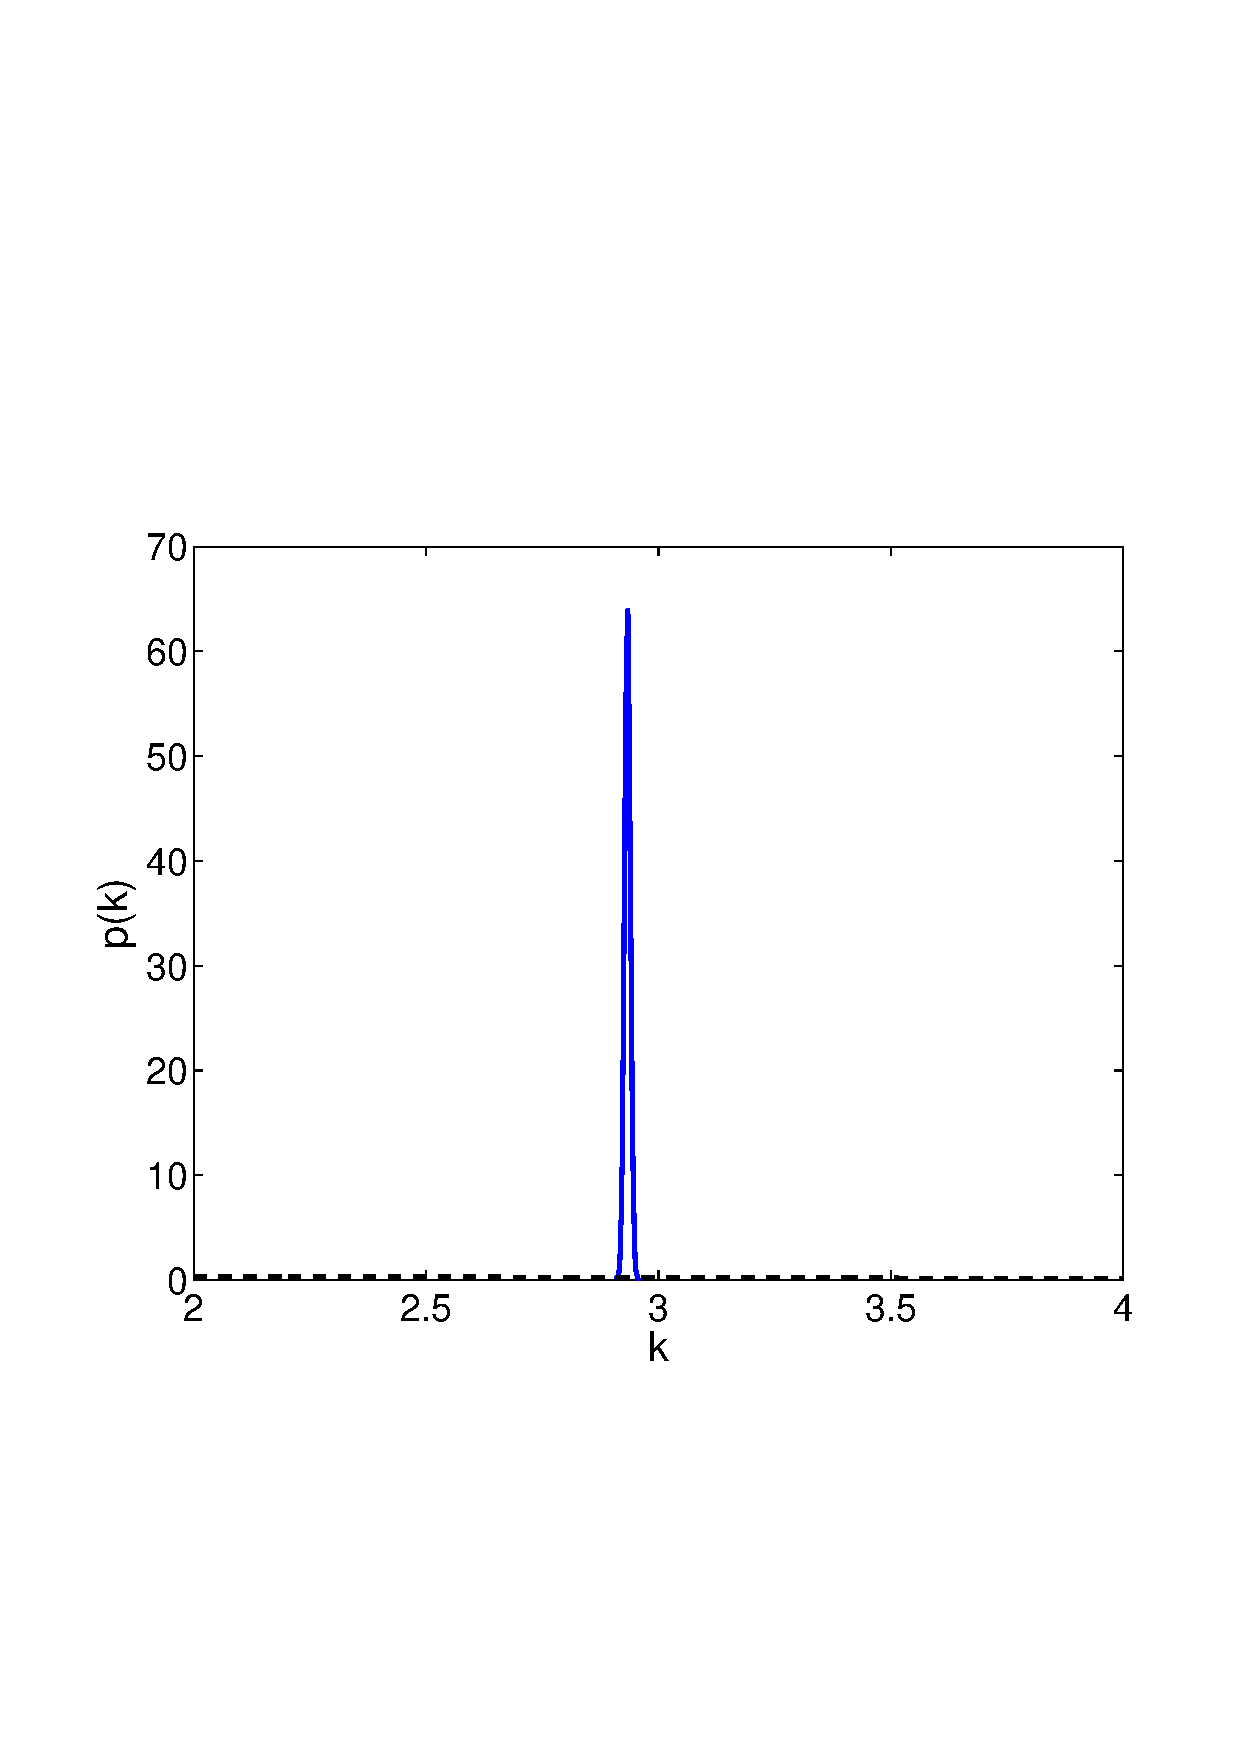
\includegraphics[width=0.45\linewidth]{k_marginal_si0.pdf}}
\subfigure[$c_o$]{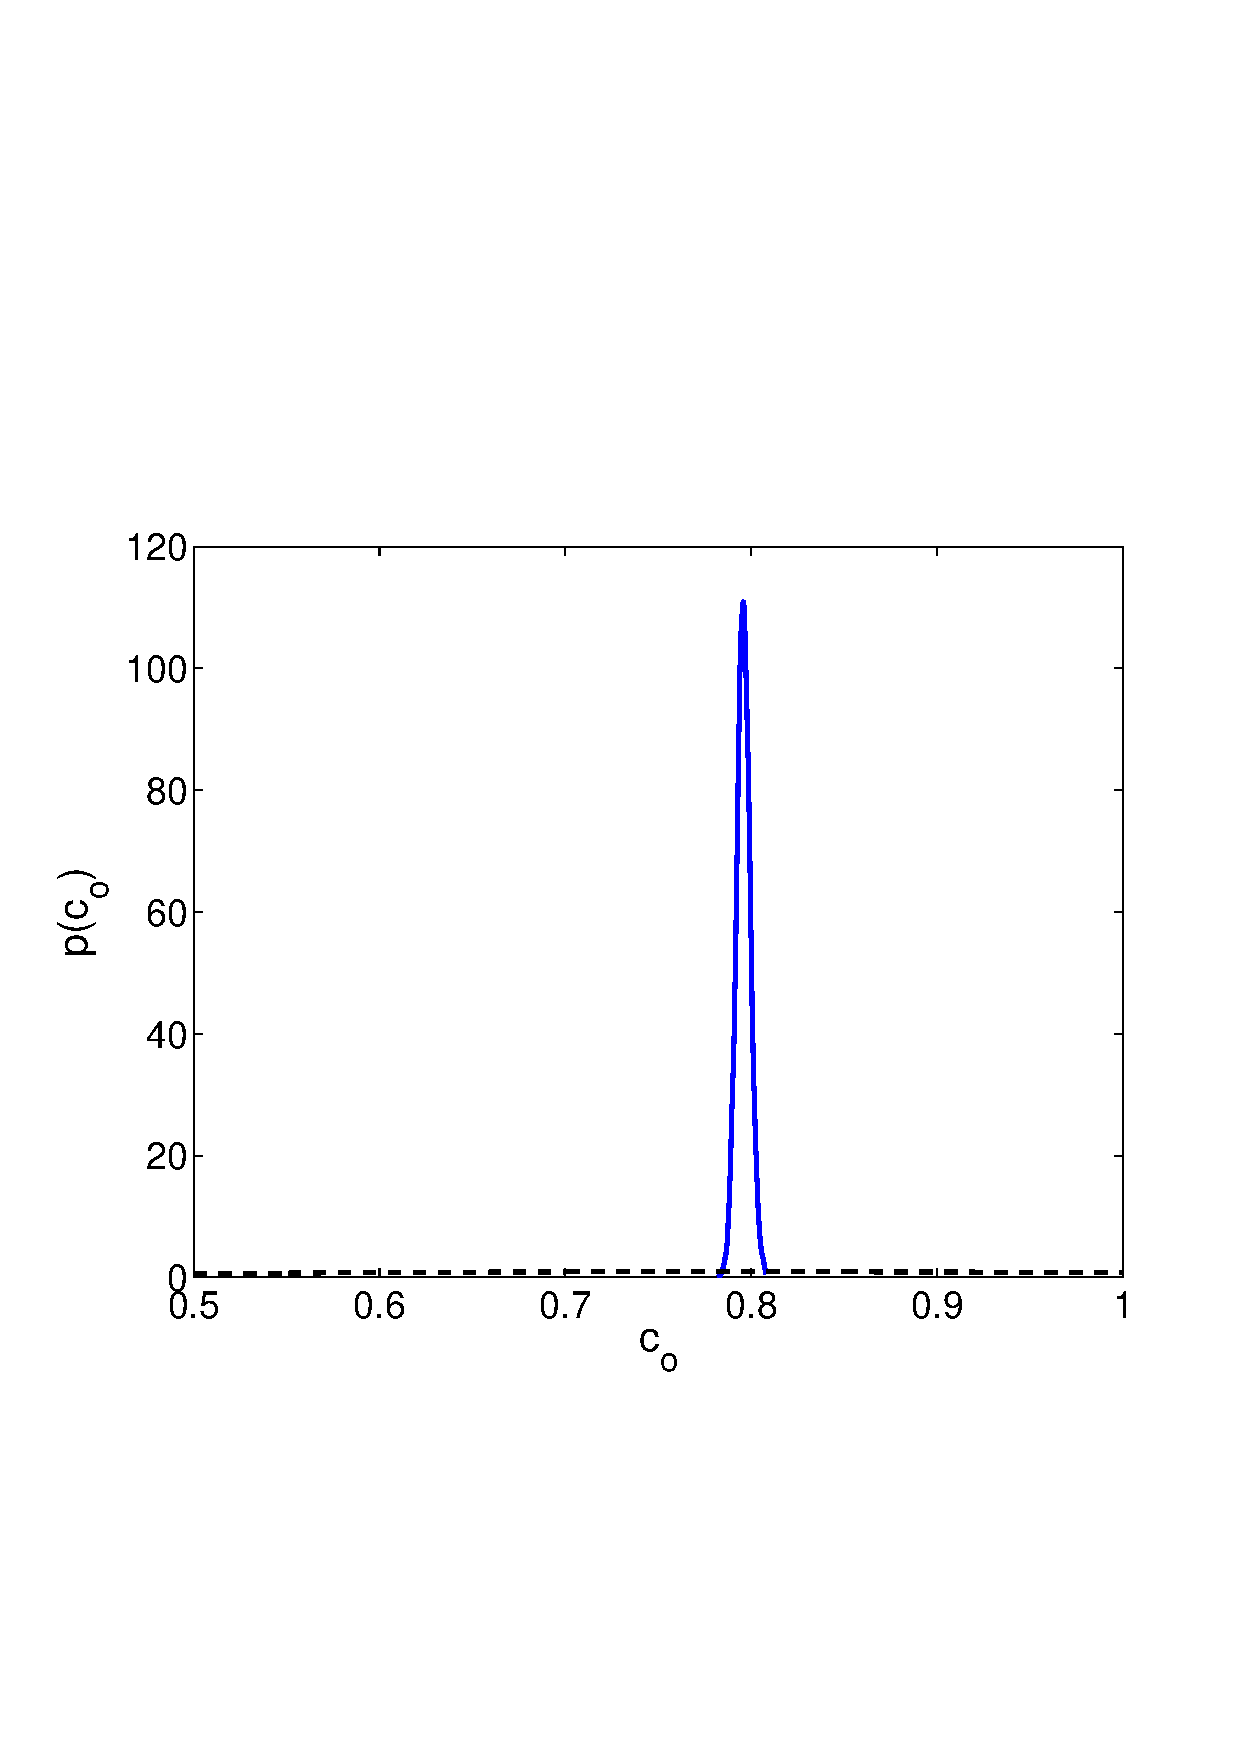
\includegraphics[width=0.45\linewidth]{cmu_marginal_si0.pdf}}
\end{center}
\caption{Marginal distributions for parameters $k$ and $c_o$.  The
  blue shows the posterior resulting from a Bayesian update of the
  prior (in black) using the calibration data set ($m=1$).}
\label{fig:si0_params}
\end{figure}
% 
Clearly, the posterior PDFs are very narrow, indicating that $k$ and
$c_o$ are highly constrained by the data.  The maximum a posteriori
(MAP) value of $k$ is (very roughly) $2.95$ (FIXME: Get better value
here... just read this off plot), which is close the true value of
$3.0$.  The MAP value of $c_o$ is approximately 0.8.  There is no
``true'' value of $c_o$ since the true damping coefficient is changing
in time.  However, this value is within true values observed for the
actual system (see Figure~\ref{fig:truth}).

\paragraph{Challenge}
The first ``challenge'' is to simply compare the output of the
calibrated model against the calibration data, as shown in
Figure~\ref{fig:si0_cal_challenge}.
%
\begin{figure}[ht]
\begin{center}
\subfigure[All data]{\includegraphics[width=0.45\linewidth]{cal_check_all_si0.pdf}}
\subfigure[$x(t = 8)$]{\includegraphics[width=0.45\linewidth]{cal_check_t8_si0.pdf} \label{fig:b}}
\end{center}
\caption{Comparison of output of calibrated model and calibration
  data.  Note that the majority of the data does \emph{not} lie
  between the $5^{th}$ and $95^{th}$ percentiles predicted by the
  model, indicating that the model assigns very low probability to the
  data.}
\label{fig:si0_cal_challenge}
\end{figure}
%
The figure indicates that none of the calibration data points lie
between the 5th and 95th percentiles given by the model.  Thus,
the model assigns very low probability to the data.  This fact can
especially be seen in Figure~\ref{fig:b}, where the red line (the data
value) is well outside of the support of the histogram computed using
the calibrated model.  While the actual error is not particularly
large (relative to the initial value for example), the error is very large
relative to the uncertainty given by the model.

Thus, for SI0, the physical model plus its uncertainty do not
plausibly describe all of the relevant observations.  In this
situation, one cannot proceed because we have demonstrated that the
uncertainty representation is unable to explain the differences
between the physical model and the data.  Thus, we cannot confidently
extrapolate to the prediciton scenario using this model, even though
the actual errors are not necessarily large.  Since we cannot explain
the observed errors, we cannot say how they extrapolate to the
prediction scenario.  Thus, the model is invalid.  Note that we only
invalidate the combination of the physical model and its uncertainty
representation.  It may be possible to improve either to get to a
valid model.

\subsection{State of Information 1}
As noted in \S\ref{sec:SI1}, SI1 does not provide enough information
to allow extrapolation, regardless of the calibration and challenge
results.  Specifically, since we are completely ignorant of the
mechanism causing the model inadequacy, we cannot form a plausible
hypothesis that would enable extrapolation, as we will for SI2.  This
is a specific incarnation of a general result, which is that without
concrete hypotheses about the mechanism causing the misfit between the
model output and the data, extrapolation cannot be done with
confidence.  While we can model the observed misfit statistically, we
cannot explain it.  In this situation, we cannot say how the errors
extrapolate to the prediction scenario.

\subsection{State of Information 2}
For SI2, we at least have enough knowledge to form a hypothesis that,
if correct, enables extrapolation to larger mass.  Specifically, our
hypothesis is that the range of $c$ increases with mass.  Thus, if we
inform a model of the variability of $c$ using the calibration data,
we would be conservative in the predicted uncertainty when using that
model at larger mass.  The predictive validation application outlined
here is intended to develop a plausible model for the variability in
$c$, inform that model, check that model (and our enabling hypothesis)
against data, and assess the prediction resulting from that model.

\paragraph{Model}
We will adopt a very simple model of the variability in $c$.  Since
$c$ must be positive, we will model $c$ using a log-normal
distribution:
%
\begin{equation*}
c = \exp( \xi ), \quad \xi \sim N(c_{\mu}, c_{\sigma}^2).
\end{equation*}
%
The parameters $c_{\mu}$ and $c_{\sigma}$ are uncertain and thus must
be learned from the calibration data. 

\paragraph{Inform} To inform these parameters (and the spring constant $k$), we use a
Bayesian update:
%
\begin{equation*}
p(k, c_{\mu}, c_{\sigma} | D_{cal}) \propto p(k, c_{\mu}, c_{\sigma}) L(k, c_{\mu}, c_{\sigma}; D_{cal}),
\end{equation*}
%
where $p(k, c_{\mu}, c_{\sigma})$ is the prior PDF, $L(k, c_{\mu},
c_{\sigma}; D_{cal})$ is the likelihood function, and $D_{cal}$ are
the calibration measurements.  The parameters $k$, $c_{\mu}$, and
$c_{\sigma}$ are taken to be independent in the prior (i.e., we have
no prior knowledge about the correlation between the parameters).
Thus, the joint prior PDF is simply the product of the marginal PDFs
for each parameter, which are chosen as follows:
%
\begin{gather*}
p(k) = \log N(1, 0.5), \\
p(c_{\mu}) = \log N(0, 0.5), \\
p(c_{\sigma}) = \log N(-1, 0.4).
\end{gather*}
%

To form the likelihood, we make two modeling assumptions.  First, the
experimental uncertainty at each measurement point is independent and
can be represented with a zero-mean Gaussian with $\sigma = 0.01$.
Second, we model each data point as being generated by an independent
draw from our random model of the damping coefficient.  Under these
assumptions, each data point is modeled as follows:
%
\begin{equation*}
p(D_i | k, c_{\mu}, c_{\sigma} ) = \int_{0}^{\infty} p(D_i | k, c) \, p(c | c_{\mu}, c_{\sigma}) \, dc,
\end{equation*}
%
where
%
\begin{equation*}
p(D_i | k, c) = \frac{1}{\sqrt{2 \pi \sigma^2}} \, \exp \left( -\, \frac{1}{2} \frac{(D_i - x(t_i; k, c))^2}{\sigma^2} \right),
\end{equation*}
%
and $\sigma = 0.01$.

Since the data points are independent in our model, the likelihood is given by
%
\begin{equation*}
L(D_{cal}; k, c_{\mu}, c_{\sigma}) = \Pi_{i=1}^{N_{cal}} p(D_i | k, c_{\mu}, c_{\sigma} ),
\end{equation*}
%
where $N_{cal}$ is the number of calibration measurements and $D_{cal}
= [D_1, \ldots, D_{N_{cal}}]^T$.

Figure~\ref{fig:si2_params} shows the marginal PDFs resulting from the
Bayesian update.
%
\begin{figure}[ht]
\begin{center}
\subfigure[$k$]{\includegraphics[width=0.45\linewidth]{k_marginal_si2.pdf}}
\subfigure[$c_{\mu}$]{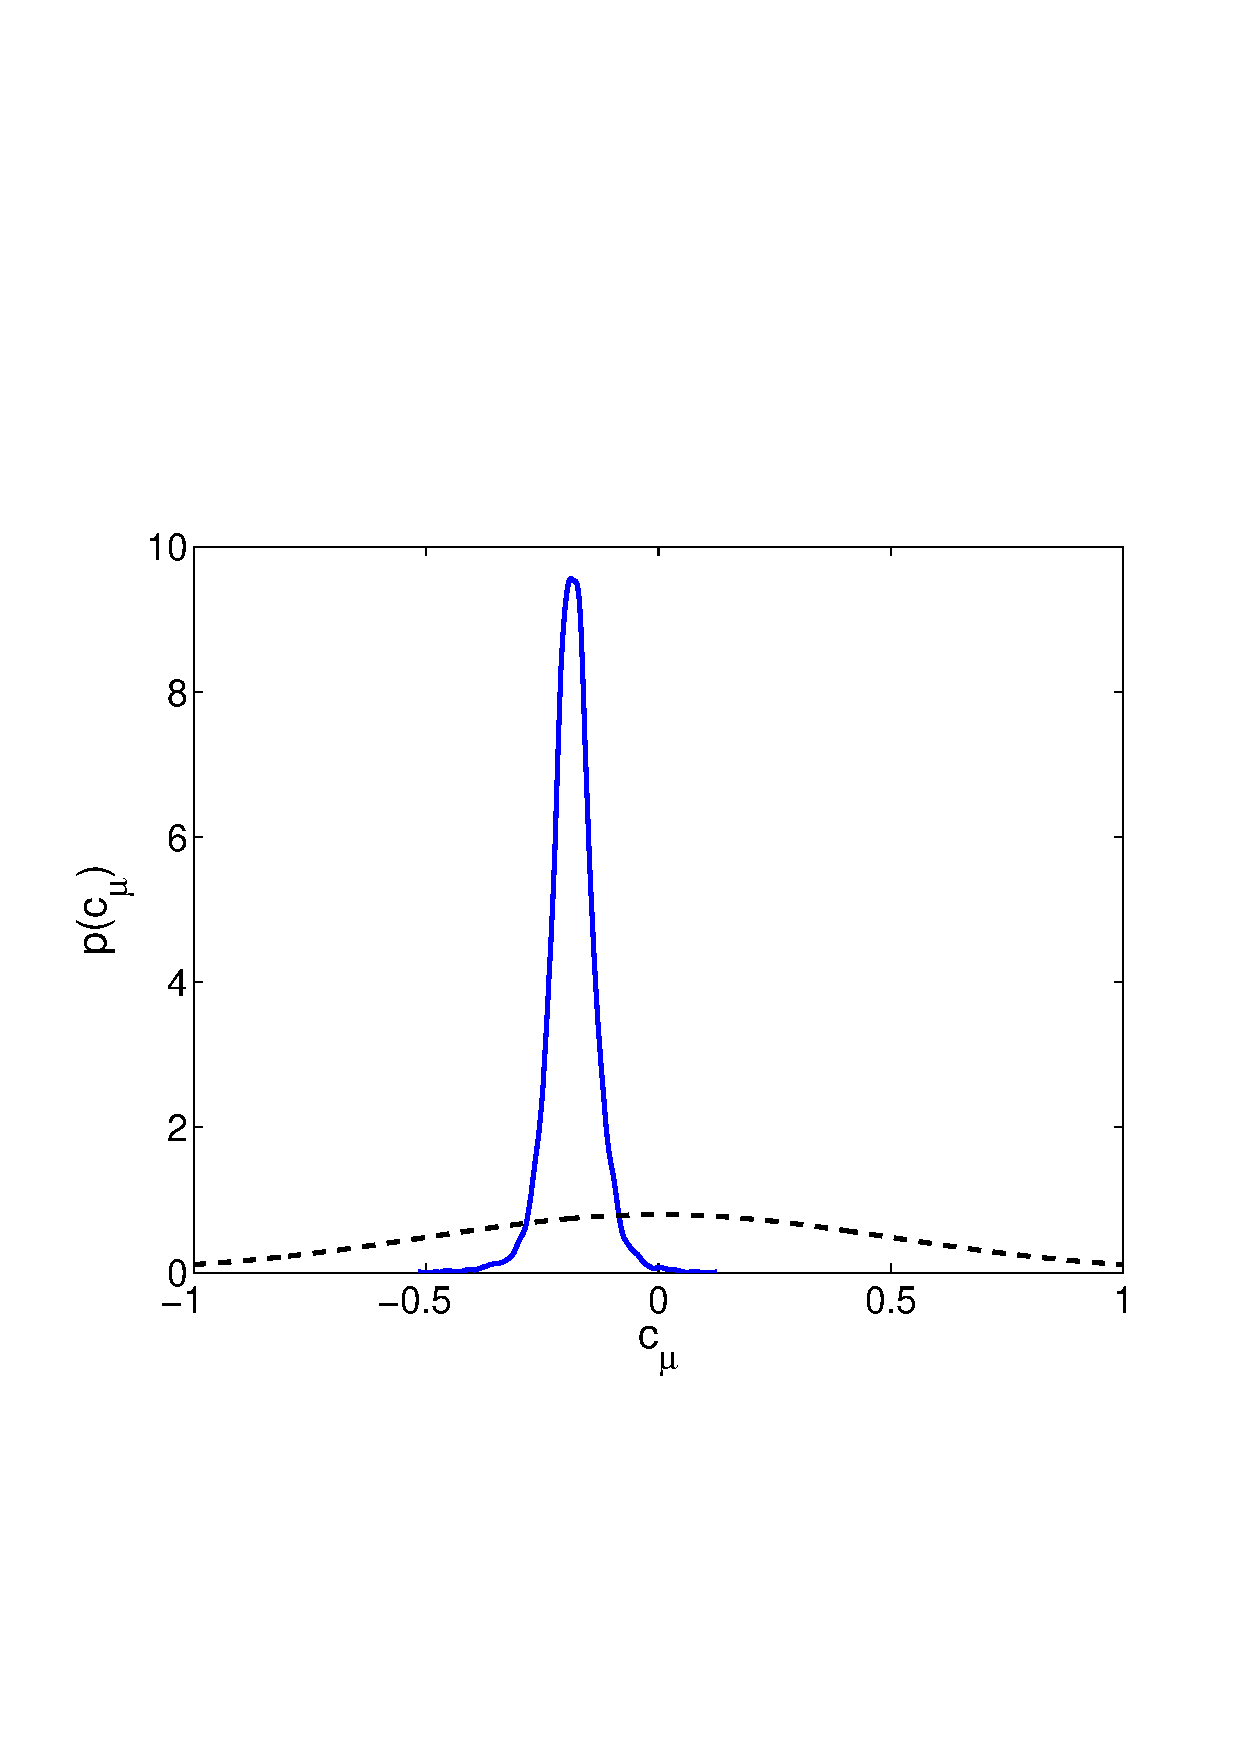
\includegraphics[width=0.45\linewidth]{cmu_marginal_si2.pdf}}
\subfigure[$c_{\sigma}$]{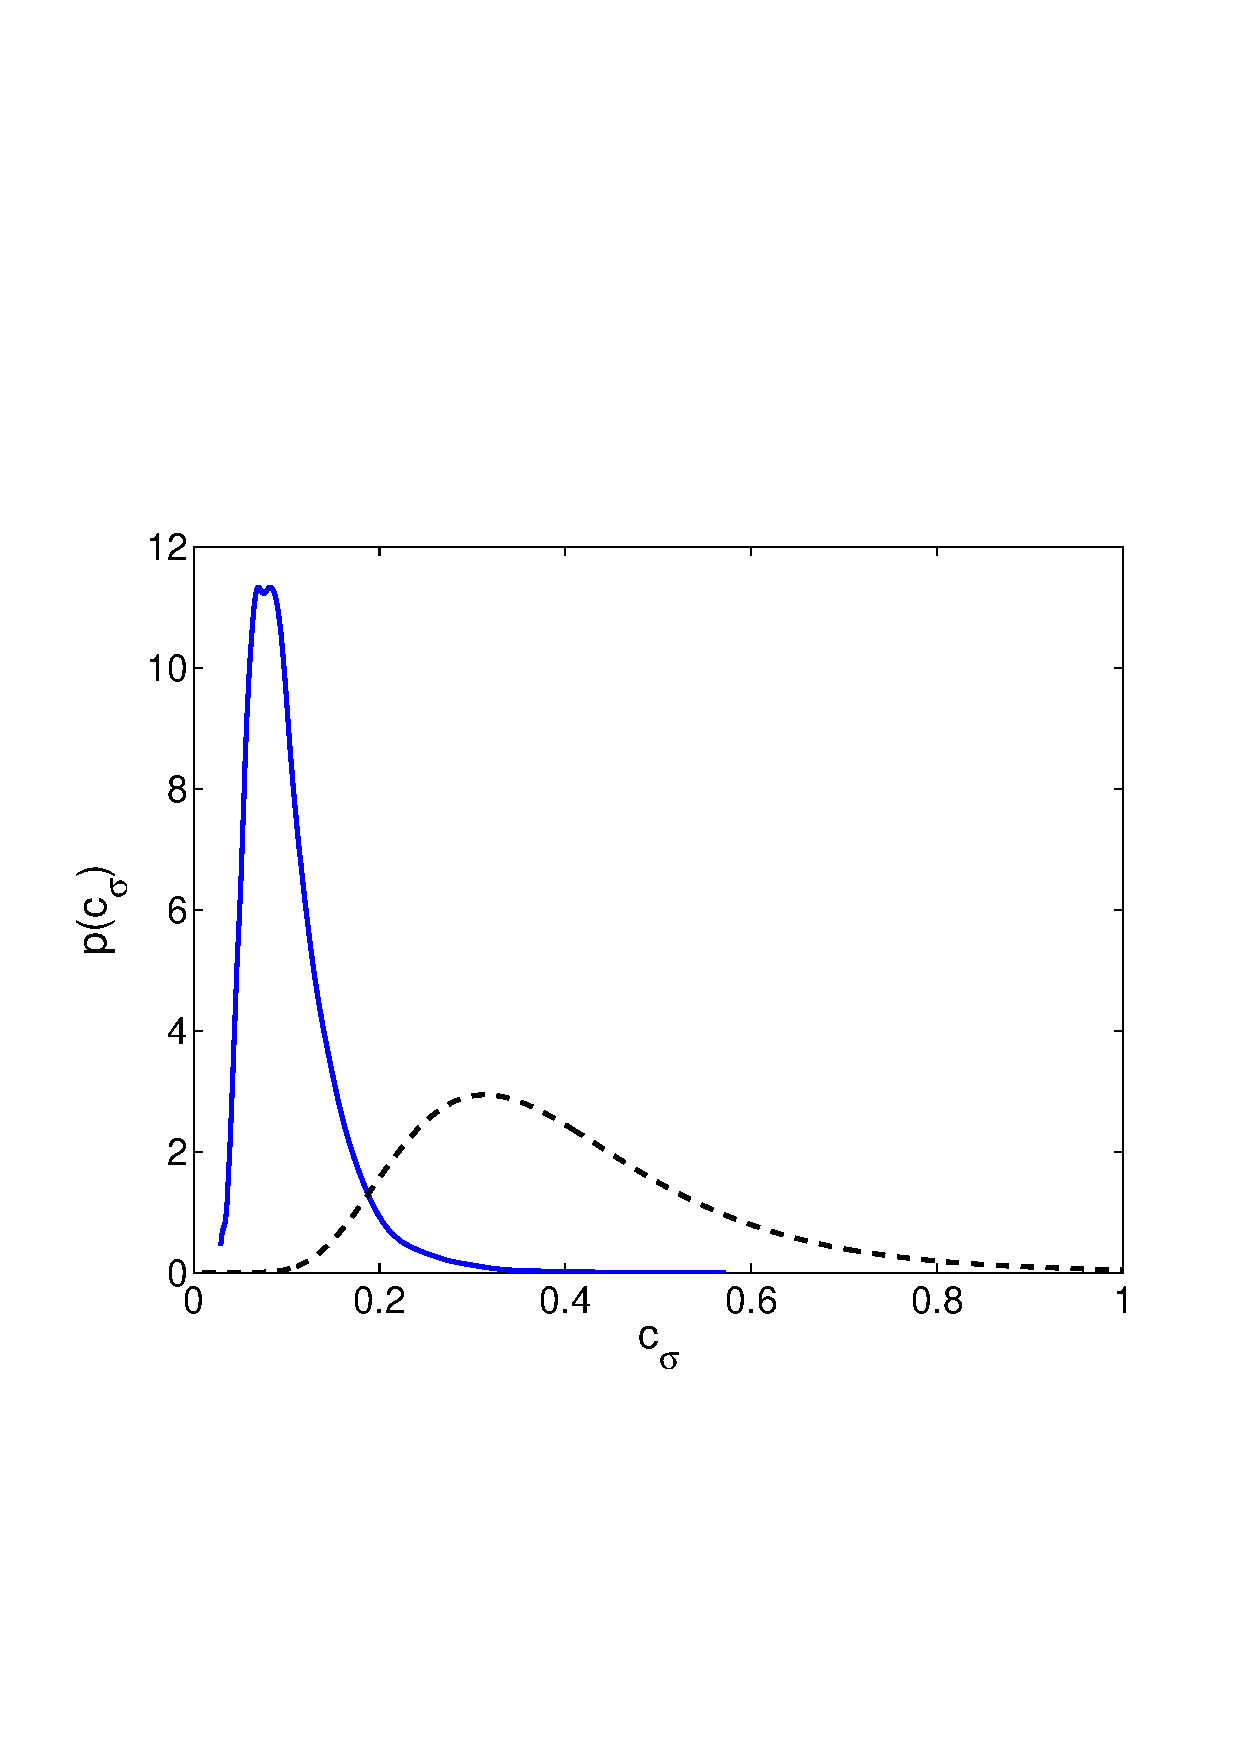
\includegraphics[width=0.45\linewidth]{csi_marginal_si2.pdf}}
\end{center}
\caption{Marginal distributions for parameters $k$, $c_{\mu}$, and $c_{\sigma}$.  The
  blue shows the posterior resulting from a Bayesian update of the
  prior (in black) using the calibration data set ($m=1$).}
\label{fig:si2_params}
\end{figure}
% 
Note that the marginal posterior for $k$ is broader than in the SI0
result and that the (unknown) true value $k = 3$ is in the support of
the posterior PDF.  To get an intuitive feel for the meaning of
$c_{\mu}$ and $c_{\sigma}$, Figure~\ref{fig:si2_csamp} shows the
log-normal distribution for $c$ corresponding to the maximum
likelhiood values of $c_{\mu}$ and $c_{\sigma}$ as well as ten draws
from the joint $c_{\mu}-c_{\sigma}$ posterior.
%
\begin{figure}[ht]
\begin{center}
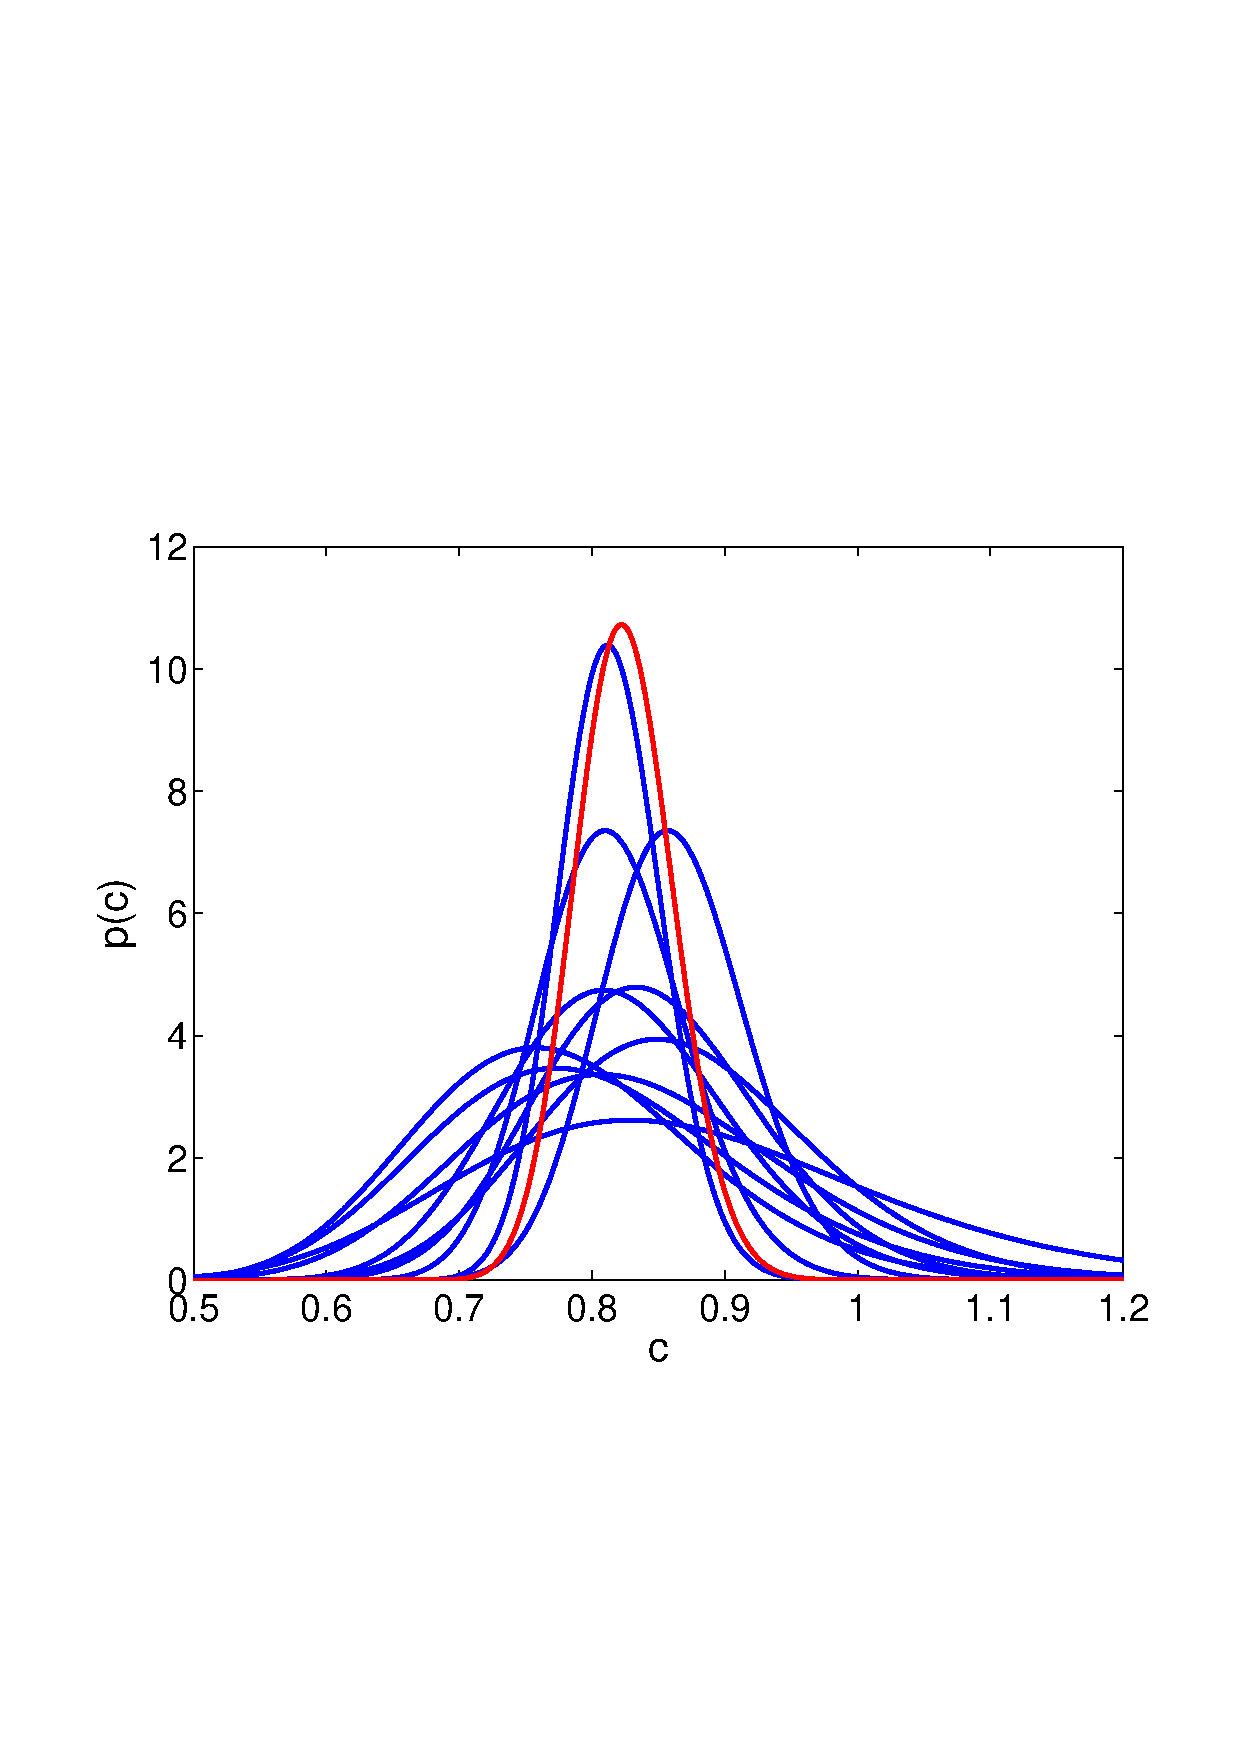
\includegraphics[width=0.45\linewidth]{csamp_marginal.pdf}
\end{center}
\caption{Log-normal distributions generated by the maximum likelihood (in red) and ten draws (in blue) of $c_{\mu}$ and $c_{\sigma}$.}
\label{fig:si2_csamp}
\end{figure}
%



\paragraph{Challenge}
Figure~\ref{fig:si2_cal_challenge} shows a comparison between the
calibration data and the output of the calibrated model.  Clearly, all
the data lies within the $5$th and $95$th percentiles given by the
model, indicating that, unlike the SI0 case, the uncertainty in the
model is sufficient to cover the calibration data.
%
\begin{figure}[ht]
\begin{center}
\subfigure[All data]{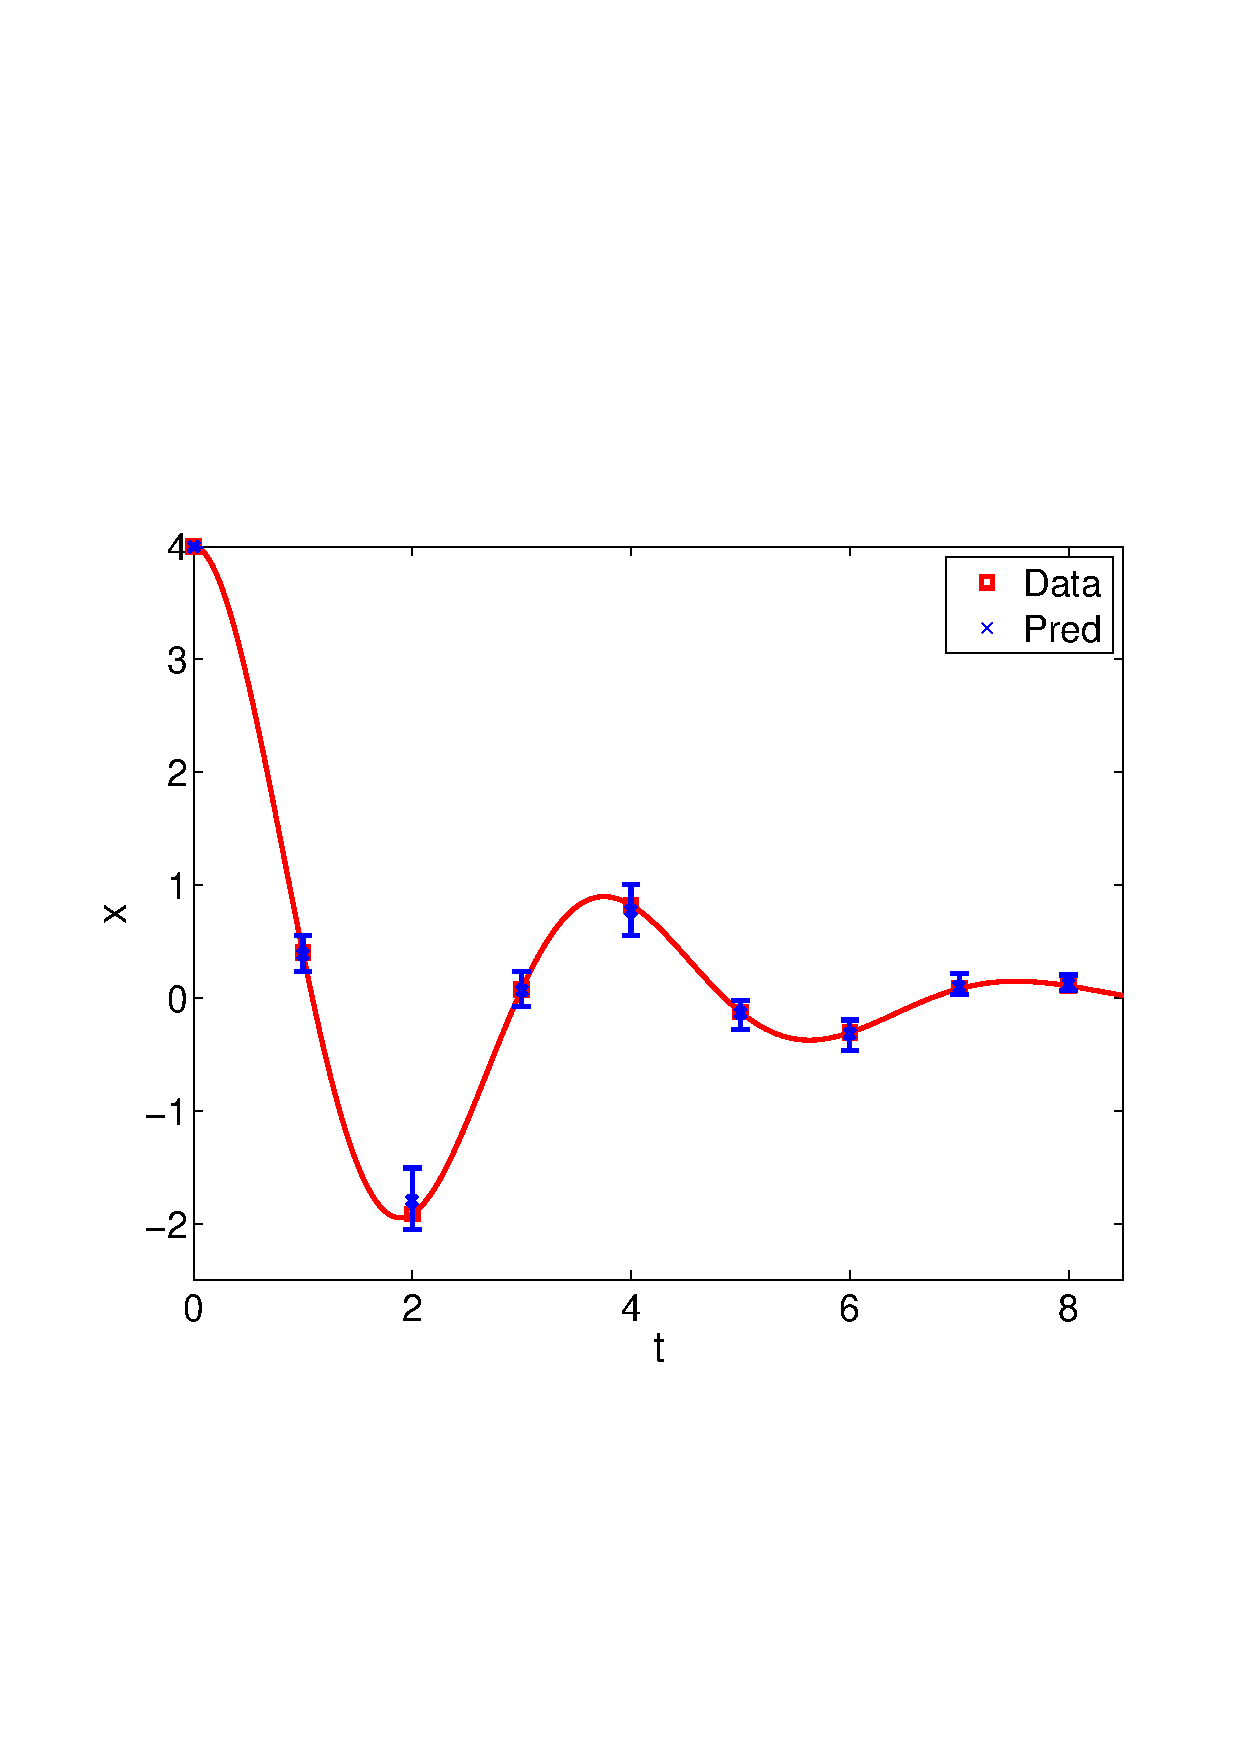
\includegraphics[width=0.45\linewidth]{cal_check_all_si2.pdf}}
\subfigure[$x(t = 8)$]{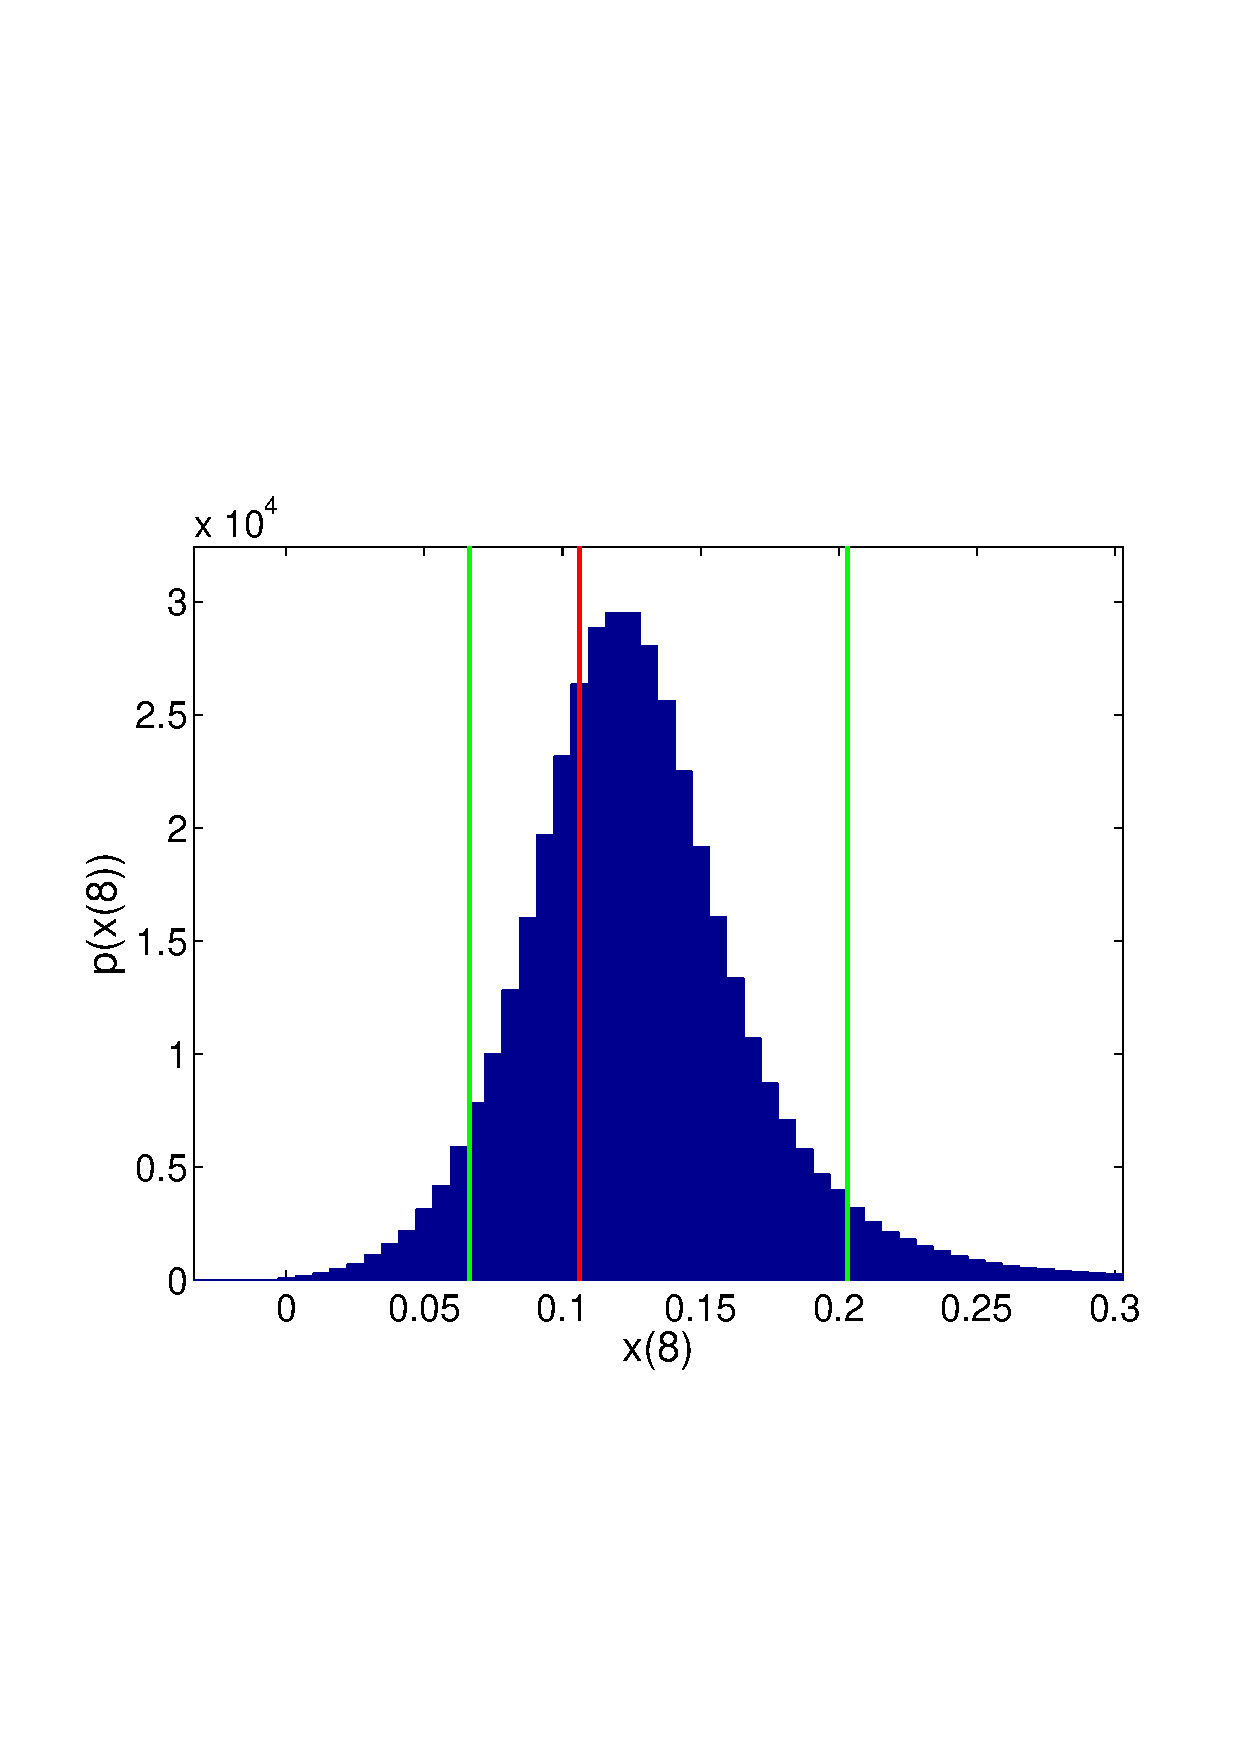
\includegraphics[width=0.45\linewidth]{cal_check_t8_si2.pdf} }
\end{center}
\caption{Comparison of output of calibrated model and calibration
  data.  Note that all of the data does fall between the $5^{th}$ and
  $95^{th}$ percentiles predicted by the model.}
\label{fig:si2_cal_challenge}
\end{figure}
% 
The same statement holds for the validation data ($m=2$), which is
shown in Figure~\ref{fig:si2_val_challenge}.
%
\begin{figure}[ht]
\begin{center}
\subfigure[All data]{\includegraphics[width=0.45\linewidth]{val_check_all_si2.pdf}}
\subfigure[$x(t = 10)$]{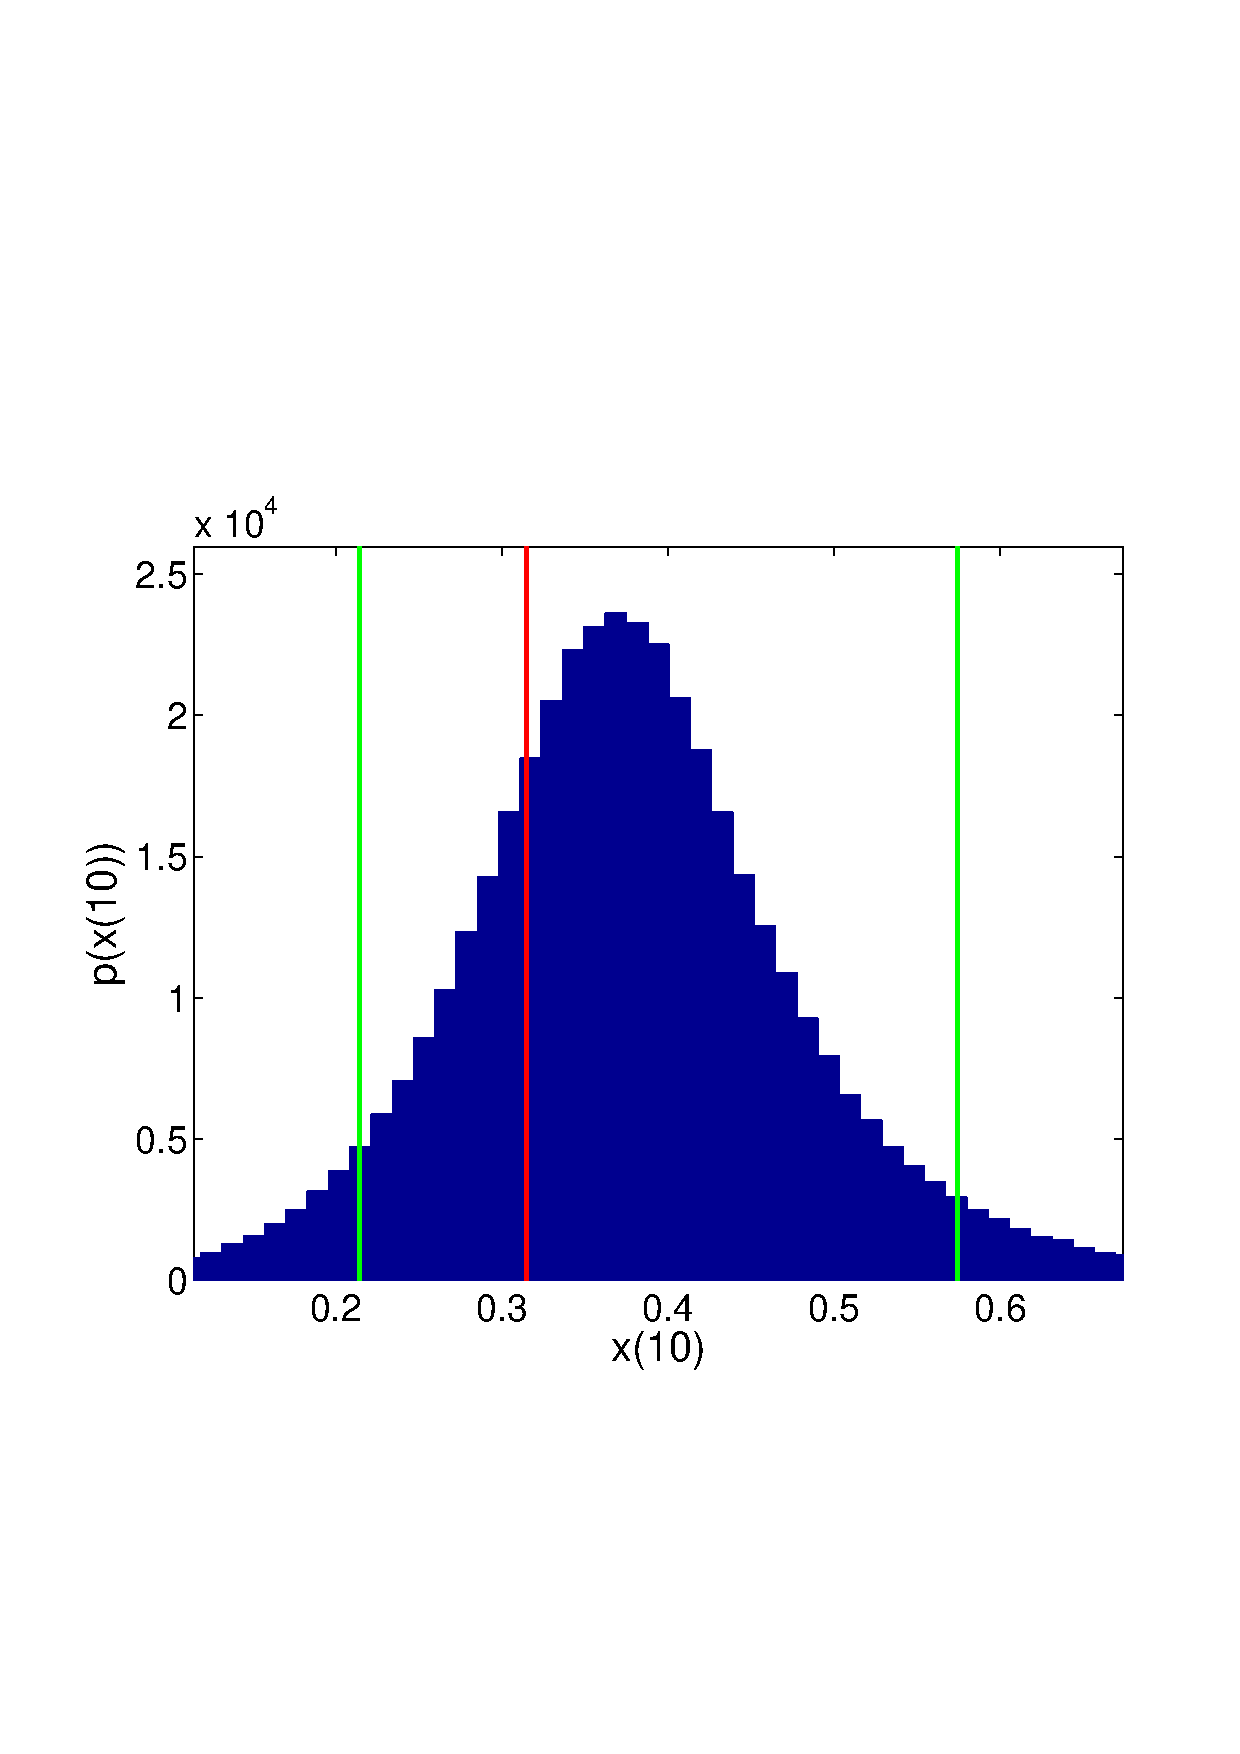
\includegraphics[width=0.45\linewidth]{val_check_t10_si2.pdf}}
\end{center}
\caption{Comparison of output of calibrated model and validation
  data.  Note that all of the data does fall between the $5^{th}$ and
  $95^{th}$ percentiles predicted by the model.}
\label{fig:si2_val_challenge}
\end{figure}
% 

{\bf TODO:} \emph{Need more challenges here to ``validate'' the
  hypothesis that variability is larger at low mass....  In
  particular, do Bayesian update with validation data and check
  results for $c$.  Should see decreasing variability (although it
  might be small).}

\paragraph{Assess}
\emph{Or, we could put that stuff as part of predictive assessment.
  Not sure what makes more sense yet.}

Having challenged our model and the hypothesis that makes
extrapolation possible, we are ready to make the prediction.  Recall
that the QoI is the maximum velocity for $m=5$.  Figure~\ref{fig:qoi}
shows the prediction given by the model as well as the true value.  
%
\begin{figure}[ht]
\begin{center}
\subfigure[Histogram]{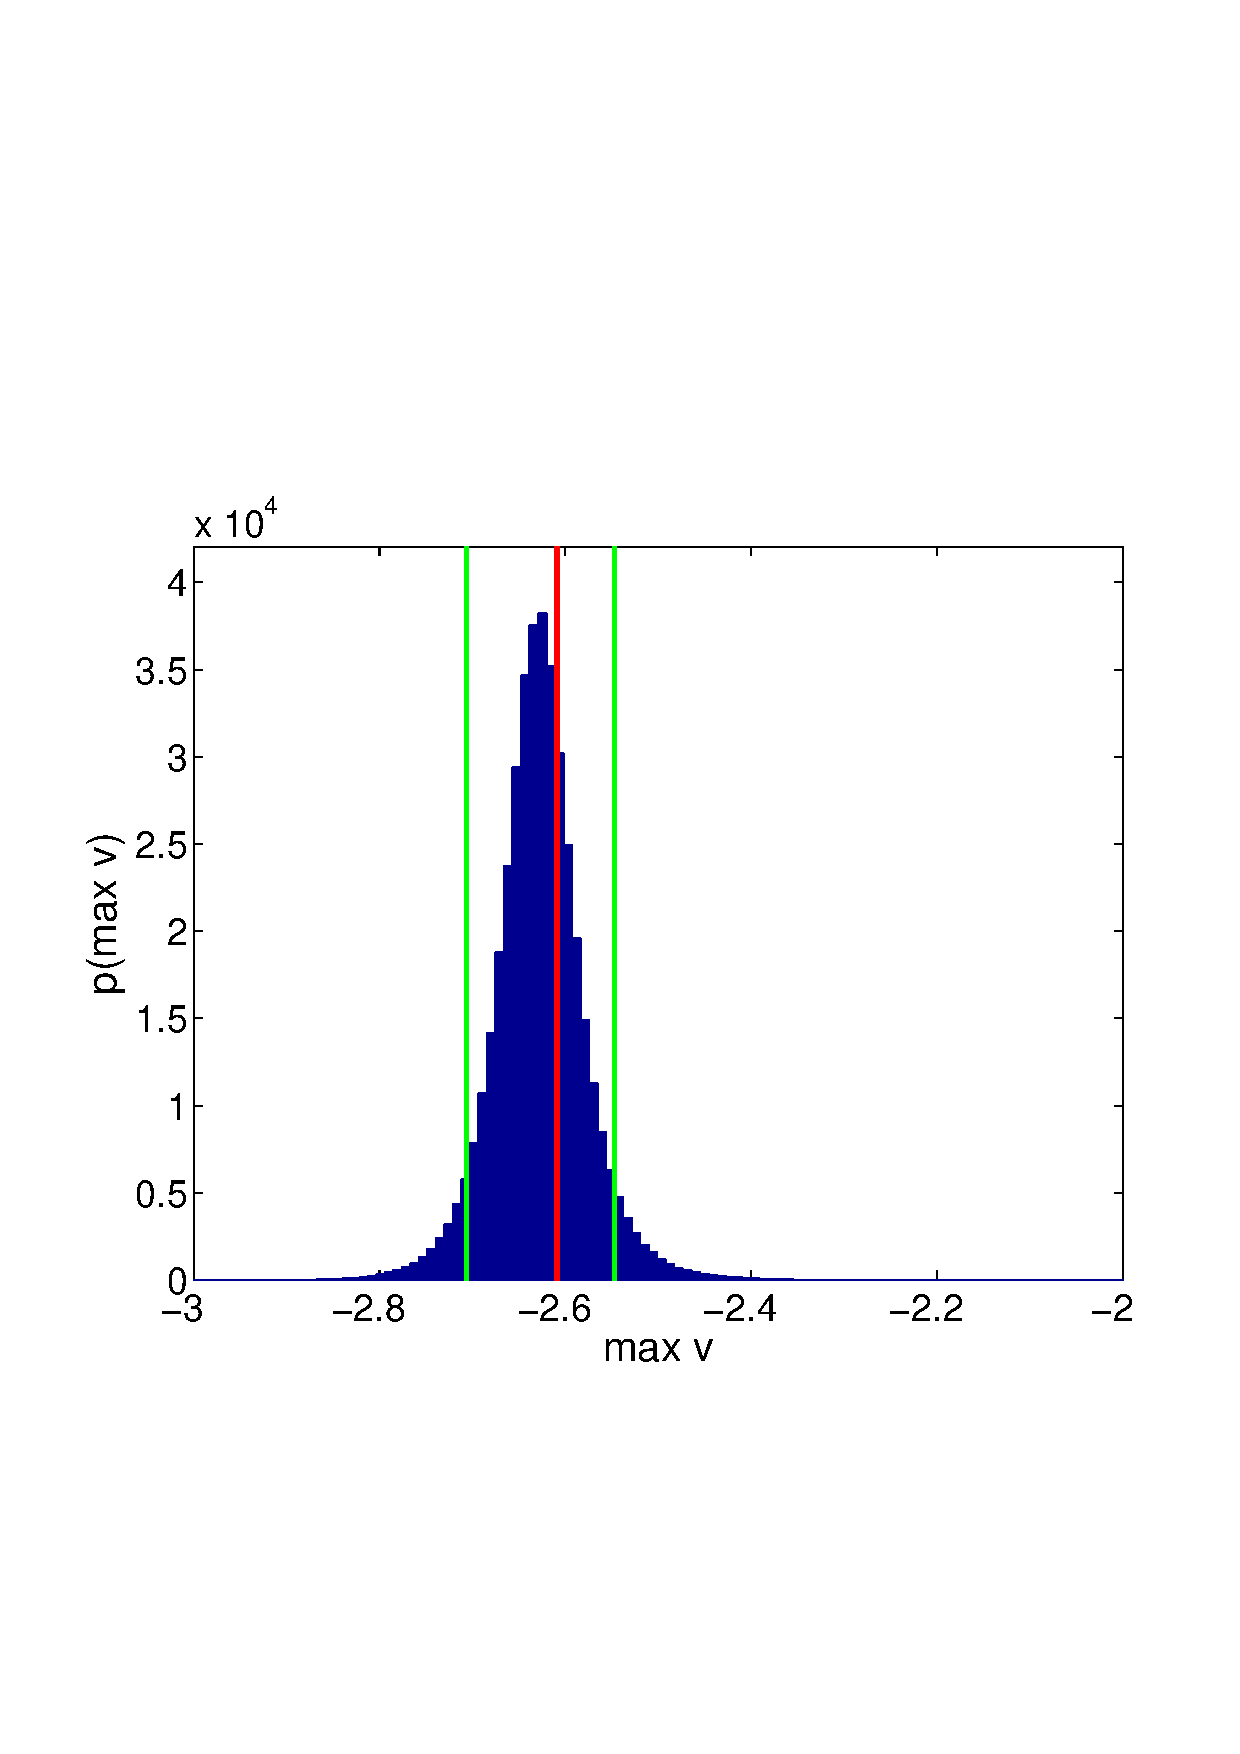
\includegraphics[width=0.45\linewidth]{qoi_hist.pdf}}
\subfigure[$v$ vs. $t$]{\includegraphics[width=0.45\linewidth]{qoi_trace.pdf}}
\end{center}
\caption{Prediction of maximum velocity for $m=5$.  The left plot shows the histogram of the model prediction as well as the actual value (in red).  The right plot shows the time history of the velocity (in red) as well as the maximum value computed by the model and its predicted uncertainty.}
\label{fig:qoi}
\end{figure}
% 
Of course, in general the true value is unknown.  It is given here
just to show that the process has led us to the correct
conclusion---i.e., the extrapolation the valid in the sense that the
truth is assigned reasonable likelihood by the model.




\appendix
\section{Truth System}
\label{app:truth}
The truth system is similar to the physical model discussed in
\S\ref{sec:phys_model}.  However, instead of having a constant damping
coefficient, the damping coefficient is a function of the temperature
of the damper fluid.  This situation is inspired by a fluid damper where the
viscosity of the damper fluid, and hence the damping coefficient,
varies with temperature.  The temperature of the fluid damper is
determined by an ODE that includes the effect of energy dissipated by
the damper and heat transferred from the damper to the surroundings,
which are assumed to have constant temperature.

The equations as as follows:
%
\begin{gather*}
m\ddot{x} + c(T) \dot{x} + kx = 0 \\
\dot{T} = c(T) \dot{x}^2 - \frac{1}{\tau}\left(T - T_0\right) \\
\end{gather*}
%
where $k$, $T_0$, and $\tau$ are constants and
%
\begin{equation*}
c(T) = \exp \left( \frac{T_0}{T} - 1 \right).
\end{equation*}
%
For all cases, the constants are set to the following values:
%
\begin{equation*}
k = 3, \quad T_0 = 20, \quad \tau = 1.
\end{equation*}
%

Figure~\ref{fig:truth} shows the position, velocity, temperature, and
damping coefficient for $m=1,2,5$.
%
\begin{figure}[ht]
\begin{center}
\subfigure[Position]{\includegraphics[width=0.45\linewidth]{reality_pos.pdf}}
\subfigure[Velocity]{\includegraphics[width=0.45\linewidth]{reality_vel.pdf}}
\subfigure[Temperature]{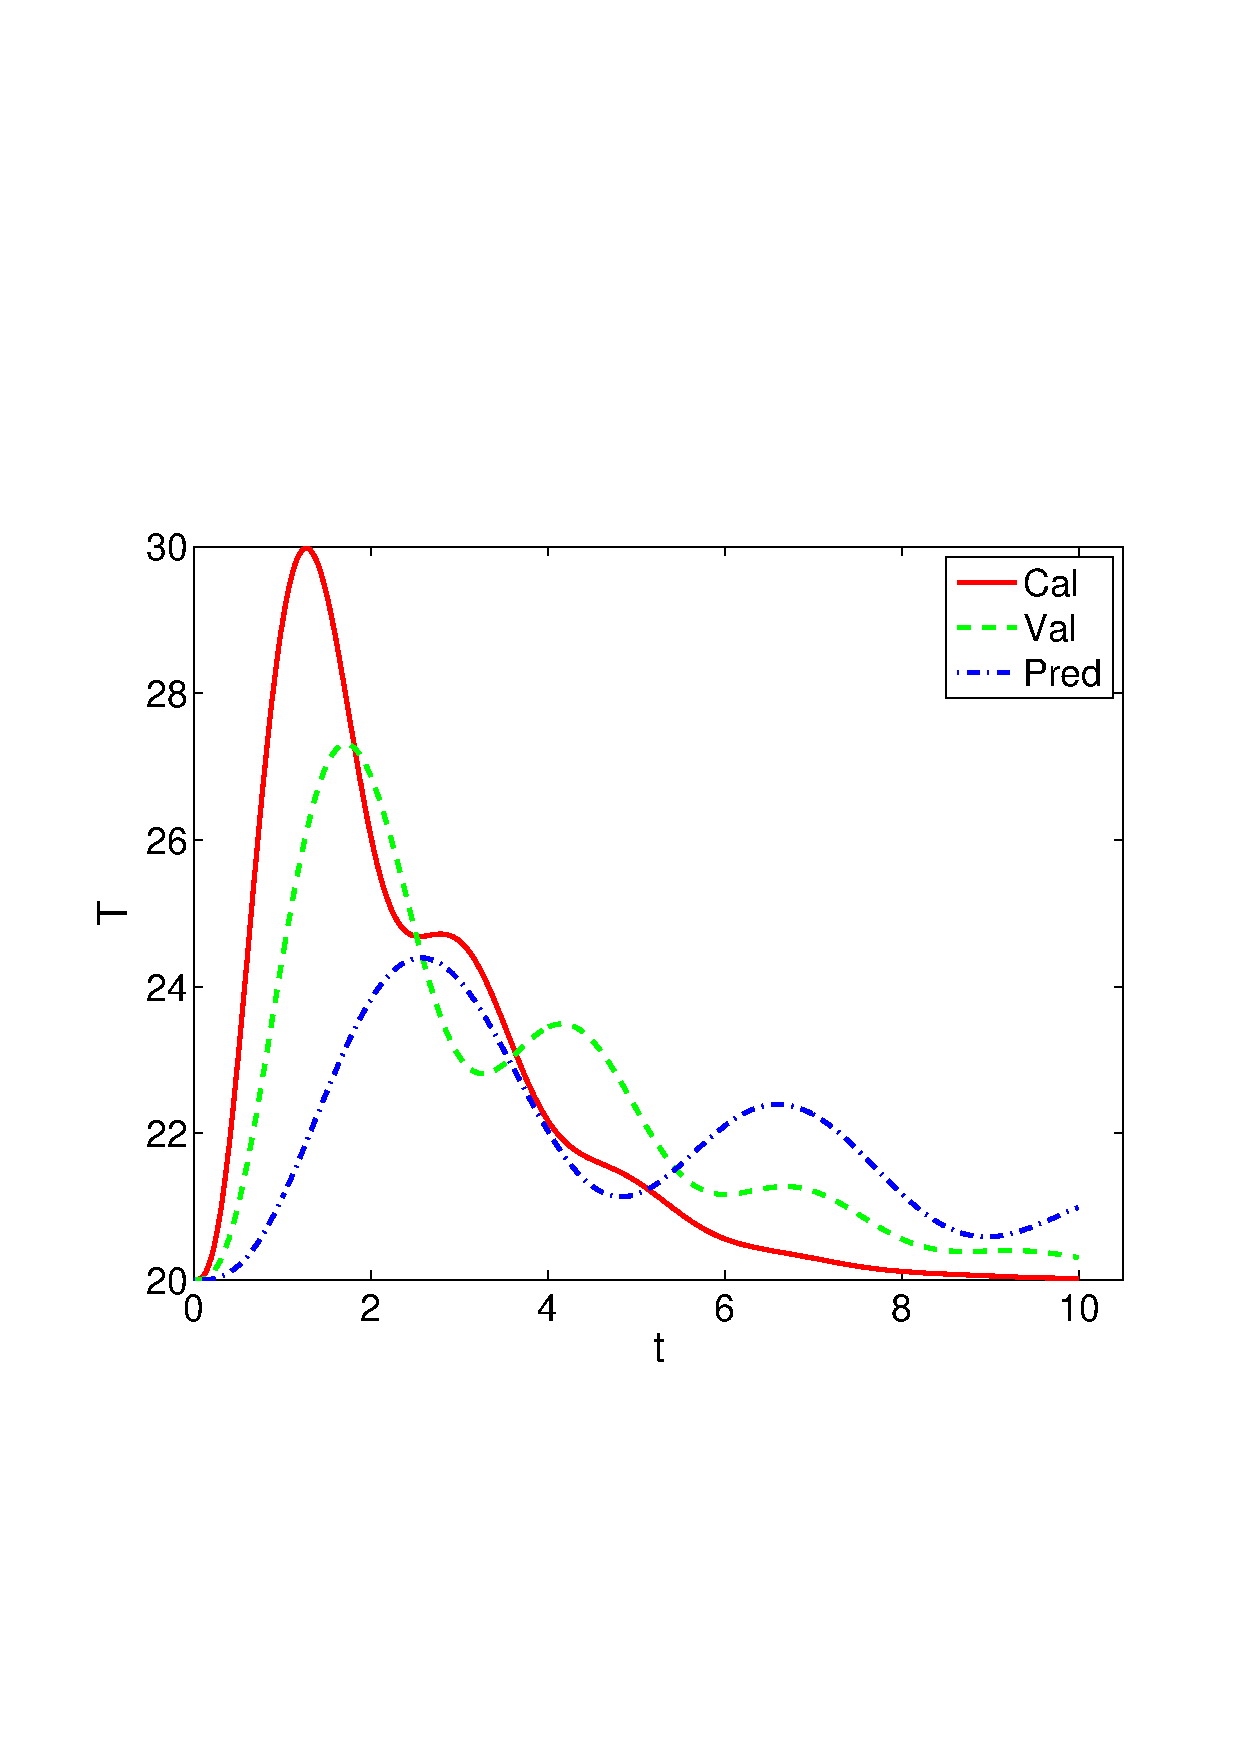
\includegraphics[width=0.45\linewidth]{reality_temp.pdf}}
\subfigure[Damp. Coeff.]{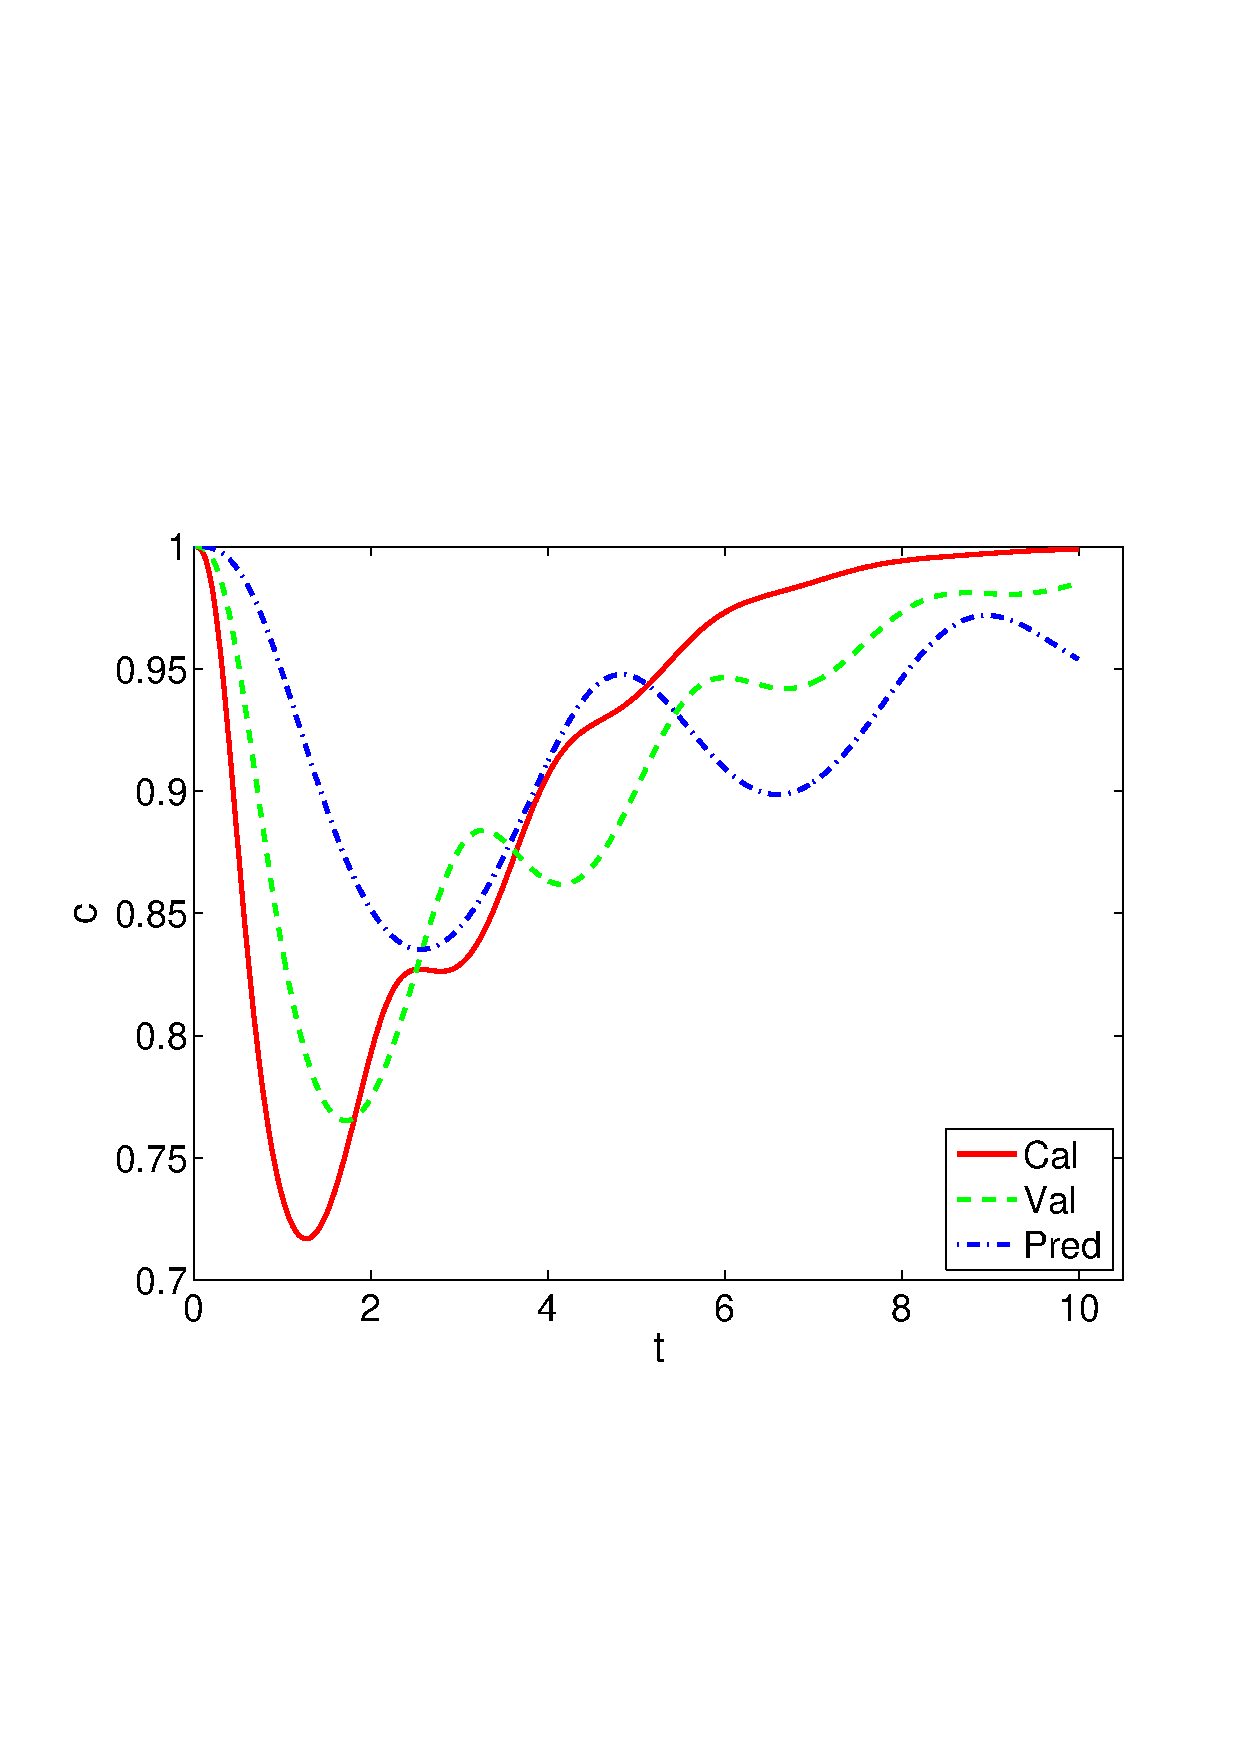
\includegraphics[width=0.45\linewidth]{reality_damp.pdf}}
\end{center}
\caption{Time history of the truth system.  Note the the range of the
  damping coefficient decreases with mass, as hypothesized in SI2.}
\label{fig:truth}
\end{figure}
%

\end{document}

